\documentclass[letterpaper,11pt]{article}
\usepackage[utf8]{inputenc} 
\usepackage{amsmath}
\usepackage{geometry}
\usepackage{graphicx}
\usepackage{tikz}
\usepackage{xcolor}
\usepackage{hyperref}
\usepackage{float} 
\usetikzlibrary{shapes.geometric, arrows, positioning}
\geometry{margin=1in}

\title{\textbf{Research Project Report}}
\author{} 
\date{\today}

\begin{document}

\maketitle
\hrulefill
%\tableofcontents
\vfill

\section{Introduction}
This document will clearly outline the advancement of the research project. Based on the Scrum and sprint methodology, I will update the document every week, including what is new and what is next.
			\begin{center}
            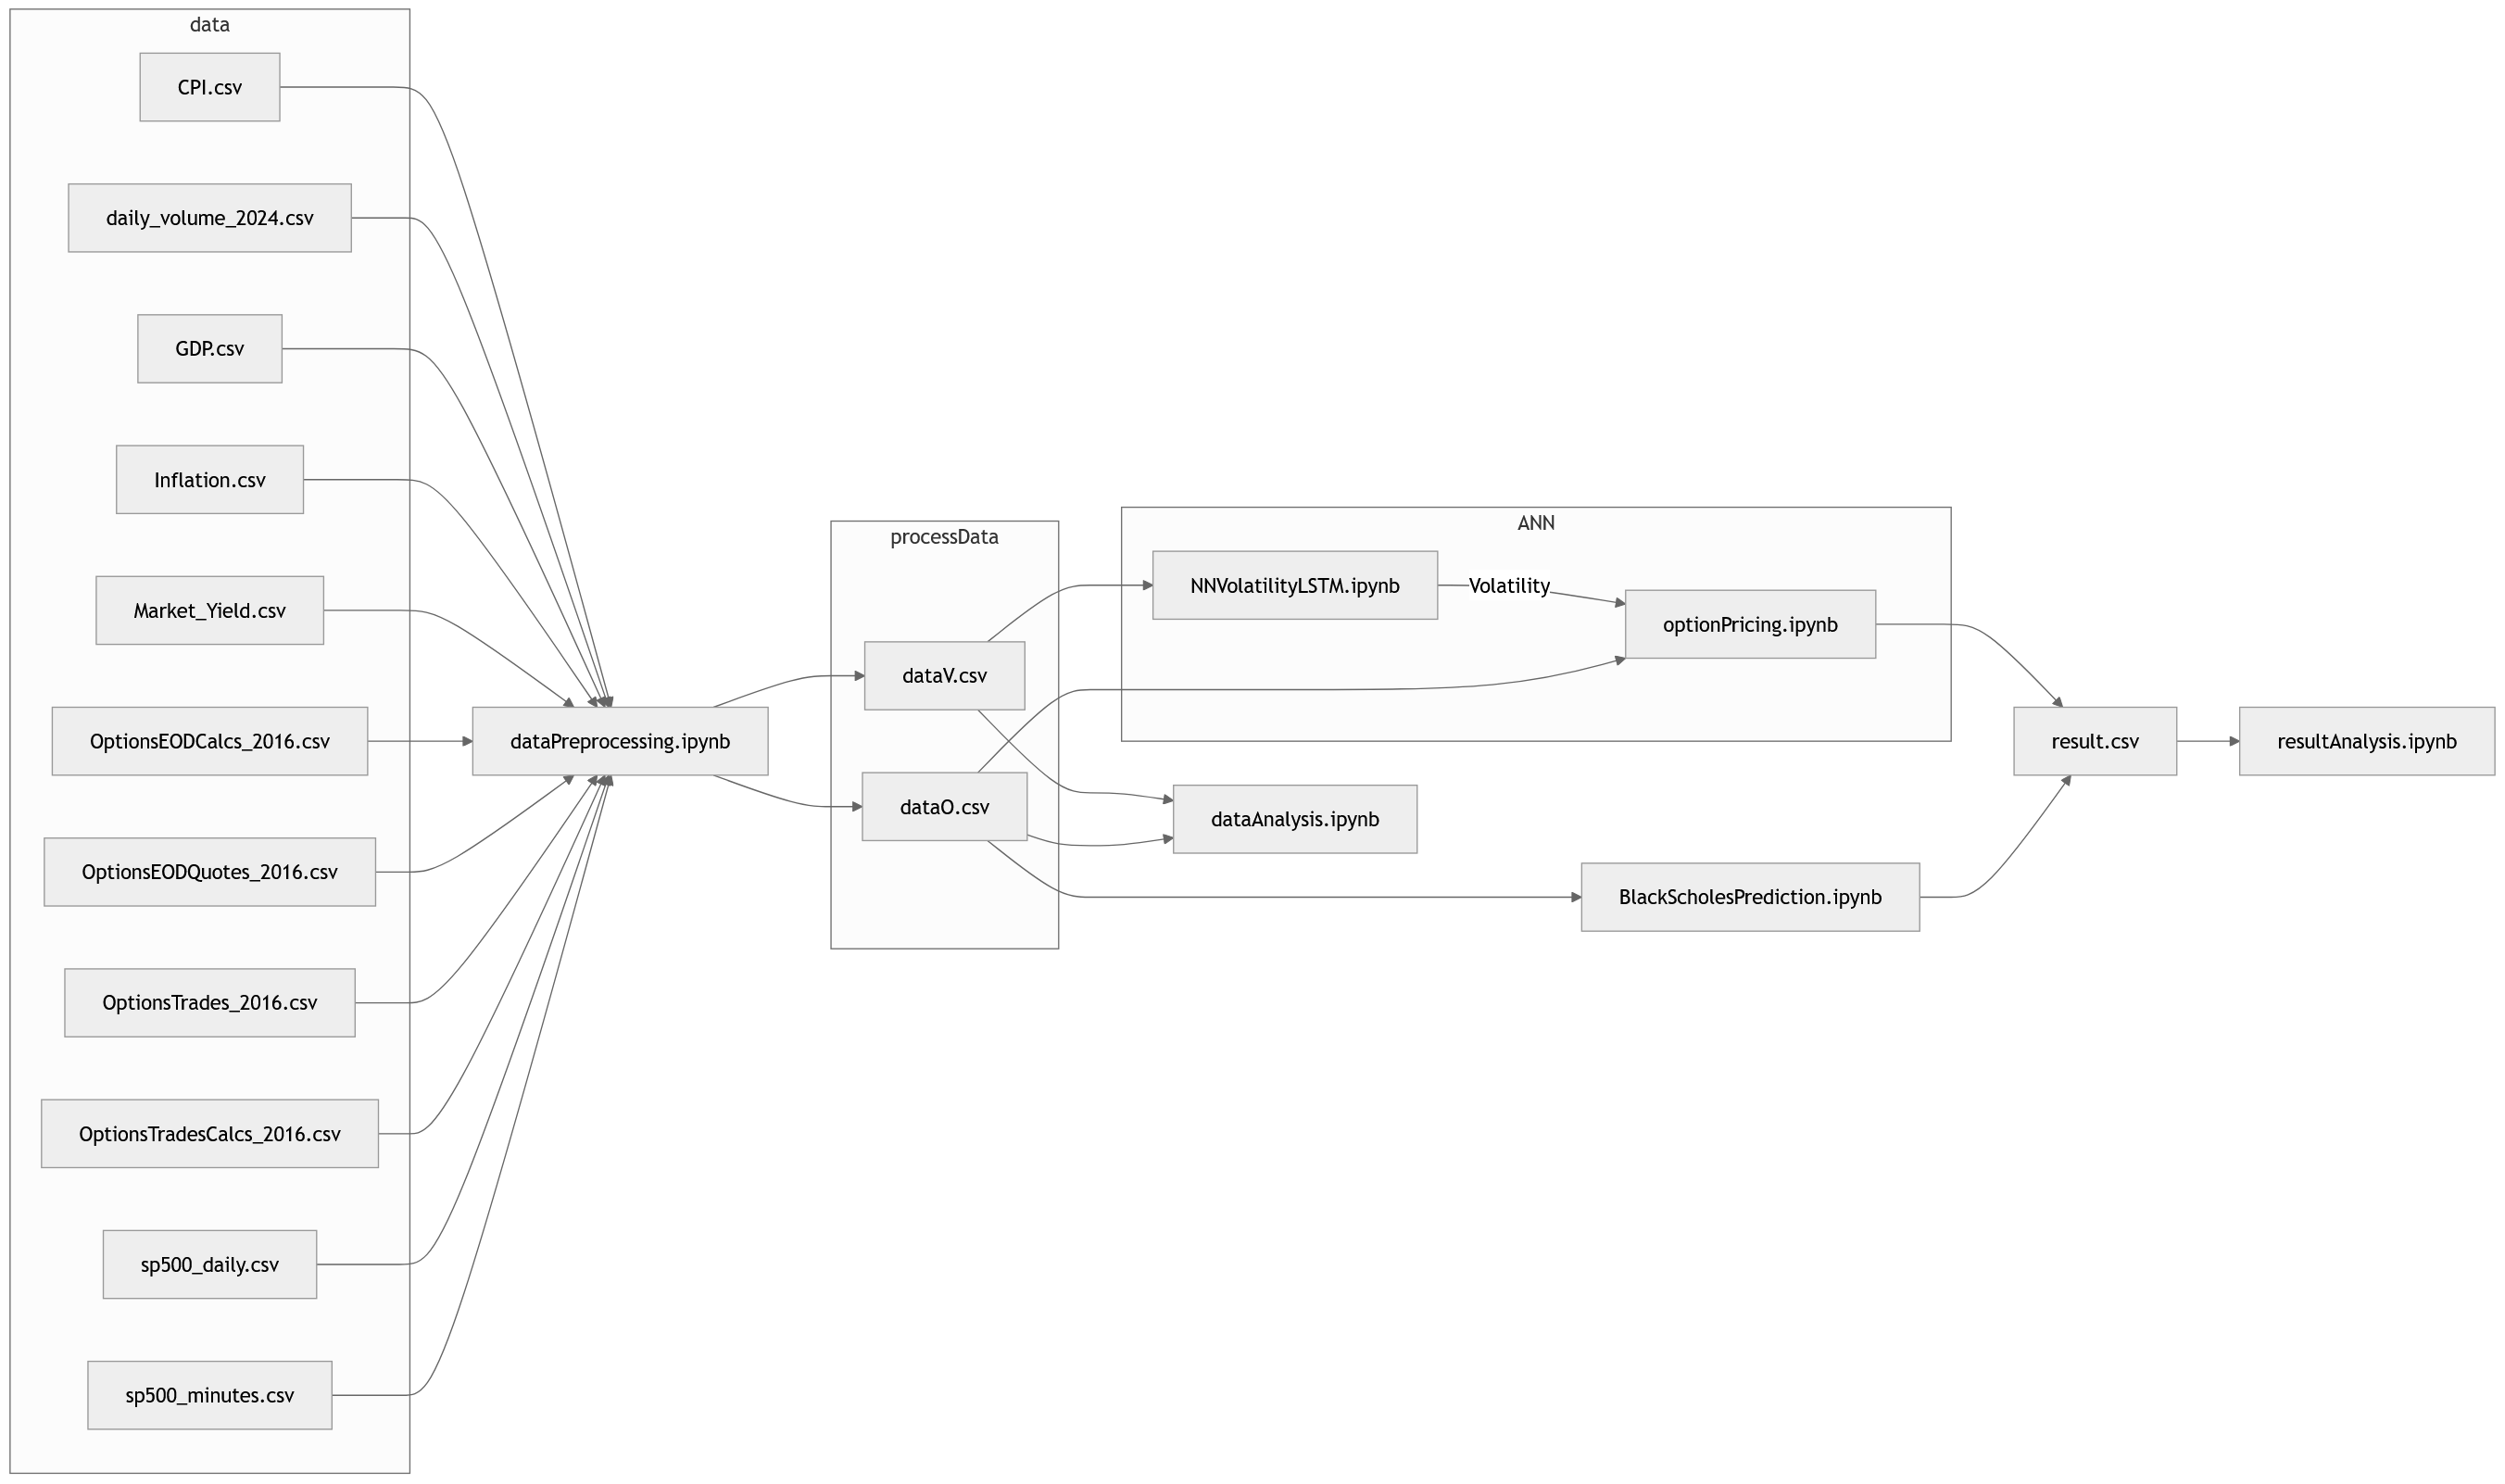
\includegraphics[width=0.9\textwidth]{img/structure.png}
            \end{center}

\newpage
\section*{Iteration 1}
\begin{flushright}
February 3, 2025
\end{flushright}
\hrule
\vspace{0.2in}

\subsection*{What Is New?}
\begin{itemize}
    \item Created and trained a ANN MLP model for option pricing, using Black-Scholes parameters to target option prices.
            
\begin{figure}[H]
  \centering
  \begin{minipage}[b]{0.45\textwidth}
    \centering
    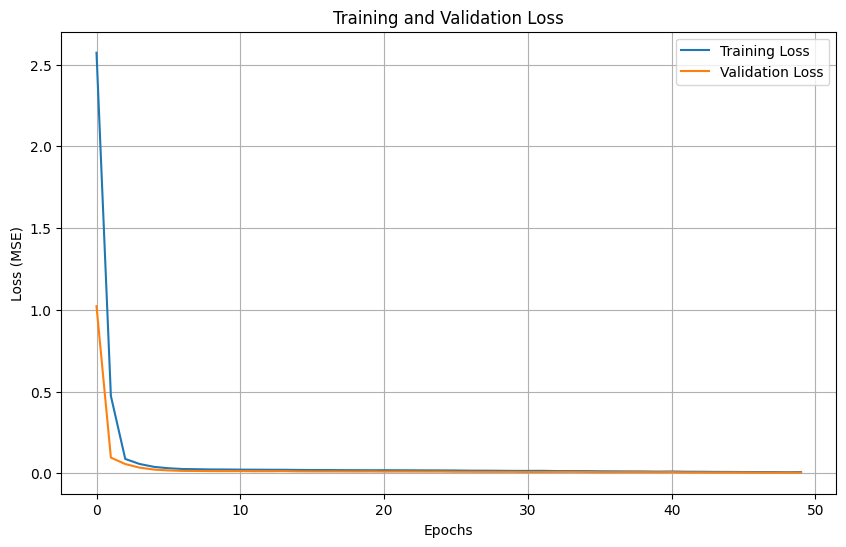
\includegraphics[width=\linewidth]{img/Loss_options_model.png} 
  \end{minipage}
  \hfill
  \begin{minipage}[b]{0.5\textwidth}
    \centering
    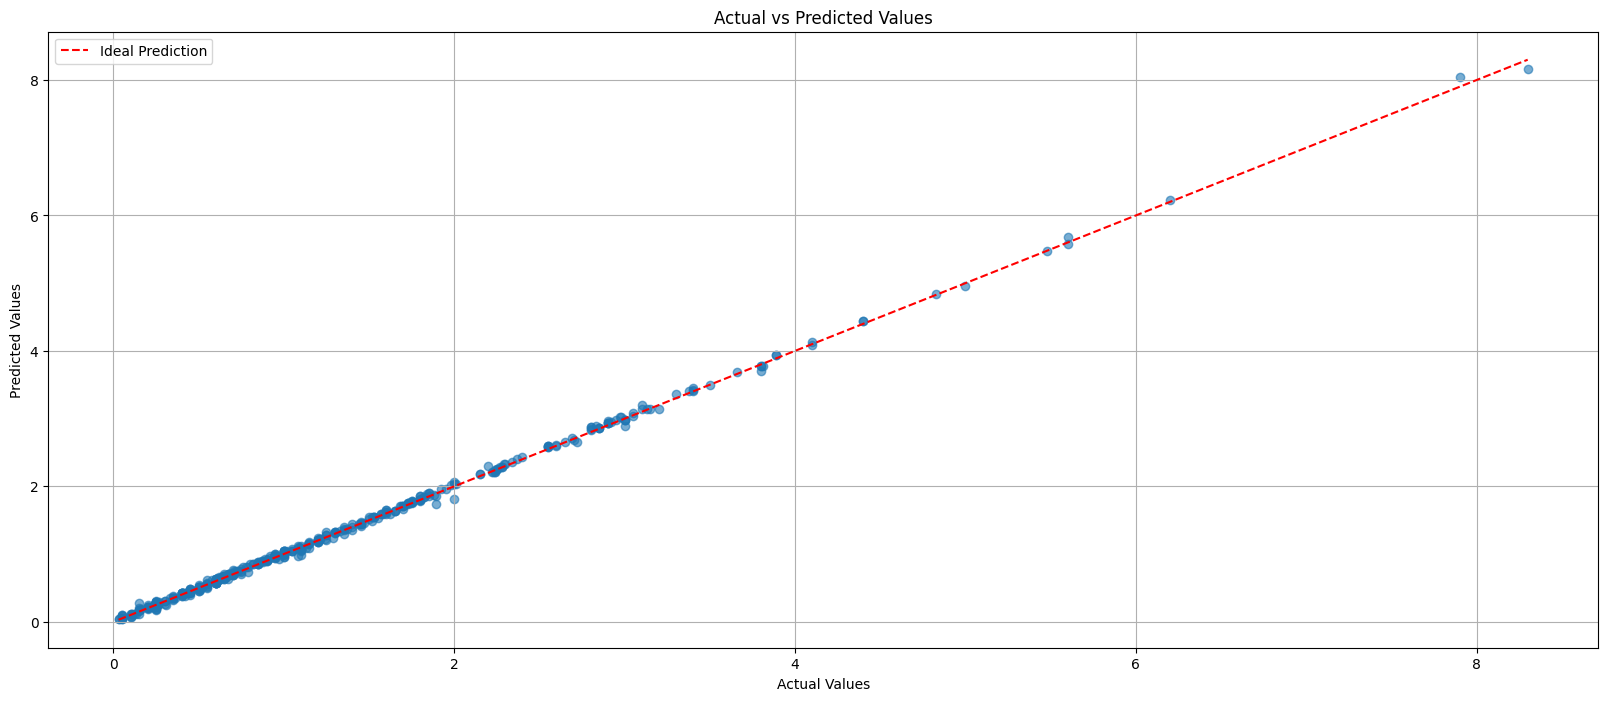
\includegraphics[width=\linewidth]{img/OPMreg.png}
  \end{minipage}
\end{figure}

    \item Compared the model's performance against Black-Scholes models:
            \begin{center}
            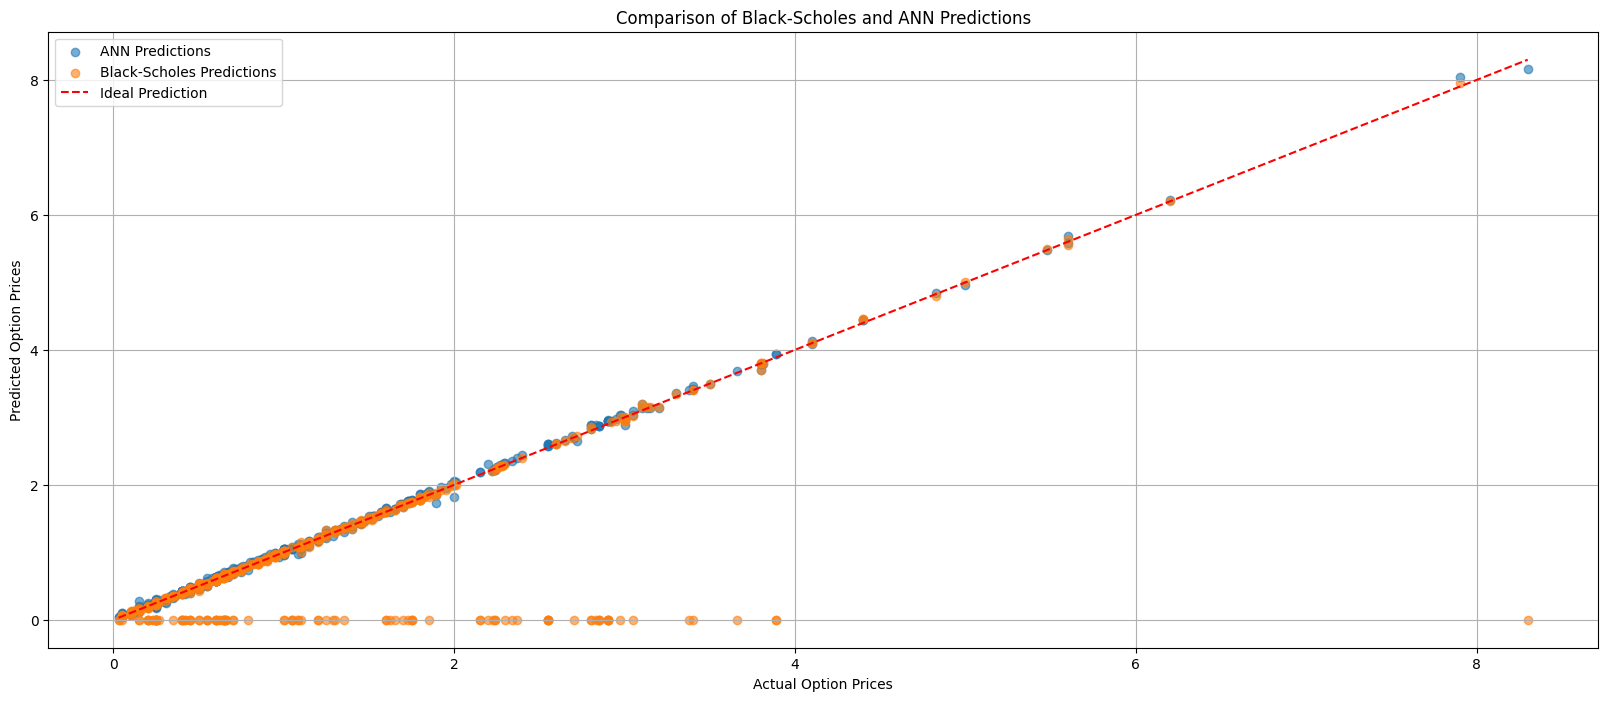
\includegraphics[width=0.8\textwidth]{img/BSvANN.png}
            \end{center}
            
    \item Started to build a custom LSTM model with NumPy. For now, I think Python allows better flexibility and development time than C++, while still maintaining decent performance using only NumPy. 
    I want the model to be compatible with TensorFlow formatting for easier use.
\end{itemize}

\subsection*{What Is Next?}
\begin{itemize}
    \item Finish the custom MLP model.
    \item Outliers suppression 
\end{itemize}

\newpage
\section*{Iteration 2}
\begin{flushright}
February 10, 2025
\end{flushright}
\hrule
\vspace{0.2in}
\subsection*{What Is New?}
\begin{itemize}
  \item First principle implementation of artificail neural network \textbf{multilayer perceptron}. Can be found here : /code\_/models/annModels.py
  \item \begin{verbatim}
  mlp = am.MLP(n_input=22, n_hidden1=64, n_hidden2=32, n_output=1)
  epochs = 5000
  learning_rate = 0.001
  
  #Training
  history = mlp.train(X_train_normalized, y_train, epochs, learning_rate)
  
  # Predict
  train_preds = mlp.forward(X_train_normalized)
  y_pred = mlp.forward(X_test_normalized)

  #---
  Final Training Loss: 0.41194406219492513
  Final Test Loss: 0.41460153925356924
  \end{verbatim}
  
  \begin{center}
    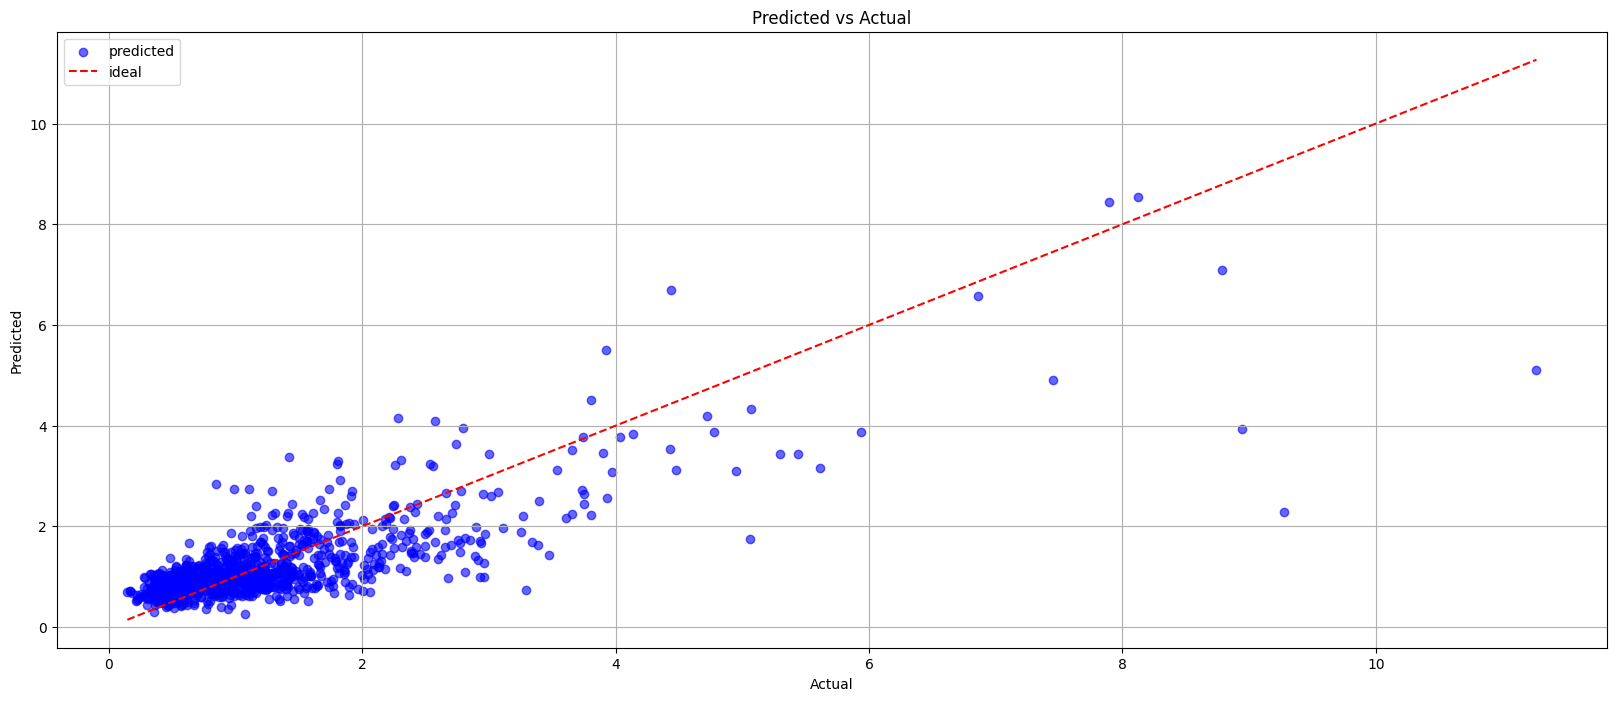
\includegraphics[width=0.8\textwidth]{img/custom_model_perf.png}
    \end{center}
\end{itemize}
\subsection*{What Is Next?}
\begin{itemize}
  \item Paramater optimization for custom model implementation ?
  \item Would a Transformer work better ? - \href{https://en.wikipedia.org/wiki/Transformer_(deep_learning_architecture)}{Wiki Transformer}
  \begin{itemize}
    \item Very likely, However, to get a working transformer model, the data volume is much more advanced than we currently use.
  \end{itemize}
\end{itemize}

\newpage
\section*{Iteration 3}
\begin{flushright}
February 17, 2025
\end{flushright}
\hrule
\vspace{0.2in}
\subsection*{What Is New?}
\begin{itemize}
  \item Finnish data gathering with scipt :/code\_/tools/getData.ipynb, all the assets data are gather in /data/stocks (around 200 symbols)
  \item Transformer implementation in progress
  \item Benchmark against LSTM model
  \item Paramater optimization for custom model implementation ?
\end{itemize}

\subsection*{What Is Next?}
\begin{itemize}
  \item Document on maths behind models (models.pdf)
\end{itemize}


\newpage
\section*{Iteration 4}
\begin{flushright}
February 24, 2025
\end{flushright}
\hrule
\vspace{0.2in}
\subsection*{What Is New?}
\begin{itemize}
  \item LSTM implementaiton in progress
  \item FFNN MLP and LSTM mathematics models
\end{itemize}

\subsection*{What Is Next?}
\begin{itemize} 
  \item Identifies specific aspect of volatility time series (mean reversion, volatility clustering, heavy tail)
  \item identifies drawback in LSTM architecture for specific financial time series
  \item Optimize model for financial time series 
  \item identify best loss function for volatility time series
\end{itemize}





\newpage
\section*{Iteration 5}
\begin{flushright}
March 3, 2025
\end{flushright}
\hrule
\vspace{0.2in}
\subsection*{What Is New?}
\begin{itemize}
  \item Data Work\begin{itemize}
    \item Compare to litterature
    \item Normalize data to improve models performances
    \item Select relevant feature to work with the model (clean confusion matrix)
  \end{itemize}
  \item Litterature about new/modify LSTM model for financial time series prediction
  \item Document on volatility model updated
\end{itemize}


\begin{center}
  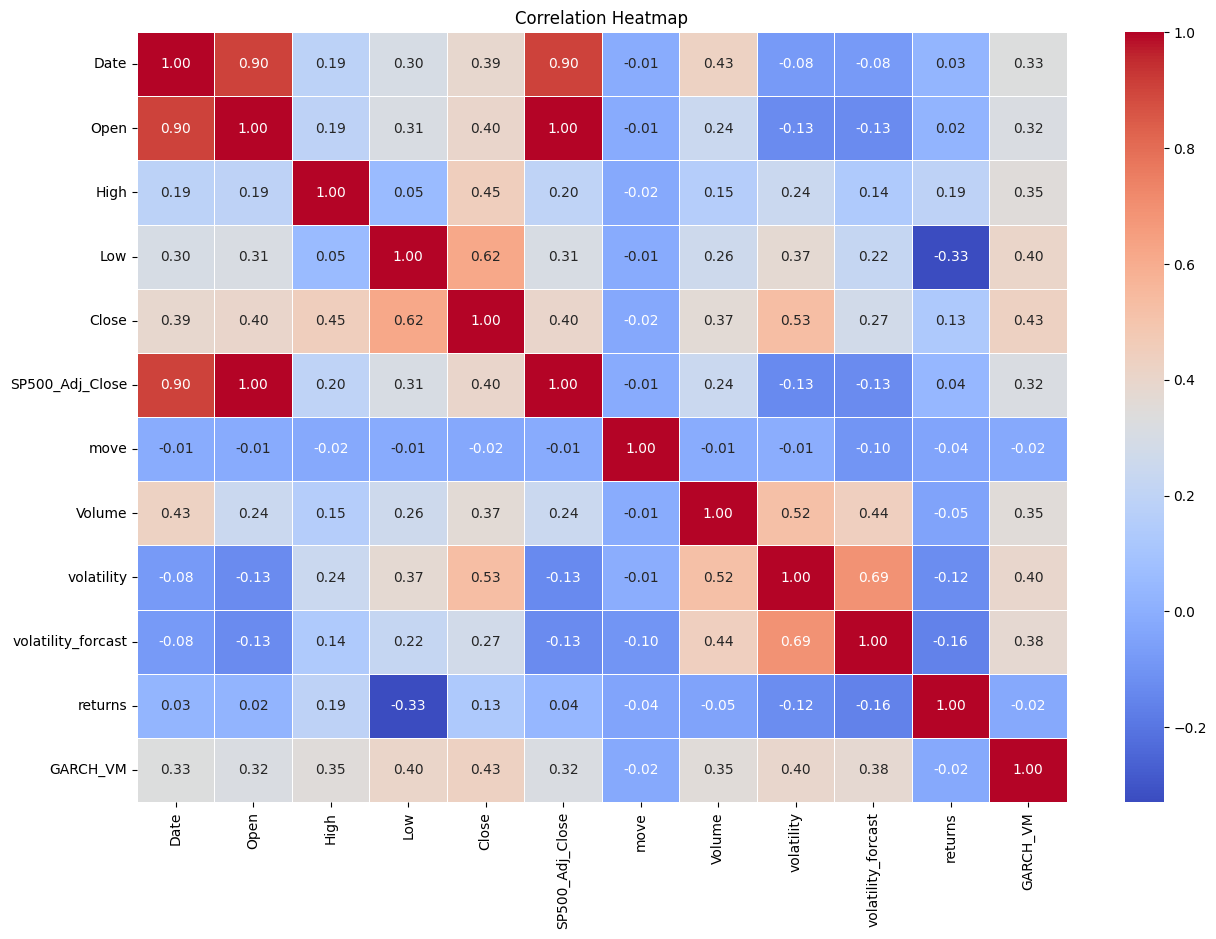
\includegraphics[width=0.7\textwidth]{img/corr_matrixS.png}
  \end{center}

\subsection*{What Is Next?}
\begin{itemize} 
  \item Improve mathematical relationship of LSTM models with litterature and financial time series properties.
  %\item 
 
\end{itemize}






\end{document}
